\documentclass[11pt]{article}
\usepackage[margin=1.15in]{geometry}
\usepackage{amsmath,amssymb,amsthm}
\usepackage{booktabs}
\usepackage{tikz}
\usepackage{microtype}
\usepackage{enumitem}
\usepackage[colorlinks=true,linkcolor=black,citecolor=black,urlcolor=black]{hyperref}

\theoremstyle{definition}
\newtheorem{definition}{Definition}
\theoremstyle{remark}
\newtheorem{remark}{Remark}

\newcommand{\Trp}{T_{\mathrm{RP}}}
\newcommand{\Trev}{T_{\mathrm{REV}}}
\newcommand{\A}{\mathcal{A}}

\title{When Failure Becomes a Signal:\\
Frustration, Refractory Time, and Collective Pattern\\
in \emph{Myxococcus xanthus}}
\author{Flyxion\\\small Independent Researcher}
\date{September 2026}

\begin{document}
\maketitle

\begin{abstract}
\noindent
Saulnier et al.\ (\textit{Nature Physics}, 2026) show that a single population of \emph{Myxococcus xanthus} can occupy two adjacent collective regimes, swarming and rippling, under one reversal rule, with the regimes distinguished only by how cells align to the surrounding matrix. Two features of that result deserve isolation. The first is that the reversal signal is not an emitted message but a residual: the discrepancy between the motion a cell would have made and the motion it achieved. The second is that the response to this residual is not a graded output but a change in when reversal is permitted at all, through a refractory period whose length is itself signal dependent. This essay states both features precisely, follows them through the paper's one-dimensional stability analysis and its two-dimensional agent model, and reads them together as a case in which an environment organizes a collective without instructing it. The paper's claims are kept separate from the interpretive frame proposed here, and the places where the evidence stops are listed at the end.
\end{abstract}

\section{Two regimes, one population}

A predatory \emph{M.\ xanthus} colony placed beside a colony of \emph{Escherichia coli} spreads over the prey and digests it. Inside the region the prey occupied, the predators eventually organize into waves that cross the surface over long distances, called ripples. Outside that region, on prey-free agar, the same cells keep swarming in streams that follow their own slime trails. The two states coexist along a sharp interface set by the prey boundary \cite{saulnier2026}.

The standard explanatory strategy has been to write one model for each state. Rippling has mostly been treated with one-dimensional continuum equations in which left- and right-moving densities reverse in response to a density signal and are prevented from reversing again during a fixed refractory period. Swarming has mostly been treated with two-dimensional agent models in which cells reverse periodically or stochastically and follow slime trails. The consequence is that the boundary between the two regimes, which is the most visible fact of the experiment, is left unexplained. It appears as a switch between programs.

The paper's central claim is that no switch is needed. Two ingredients suffice: alignment of cells to the extracellular matrix (ECM), which differs between the two regions, and the ability of cells to resolve congestion by reversing, with a refractory period that can be tuned. Everything else is held fixed. The remainder of this essay is about why that is a stronger claim than the familiar remark that simple rules produce complex behavior, and what exactly the two ingredients are.

\section{What was measured}

The empirical starting point is a set of single-cell observations in adjacent rippling and swarming fields. Three matter for what follows.

First, alignment differs. Nematic order stays high over long distances in the rippling field and falls to near zero within a few cell lengths in the swarming field. The reversal-defective \emph{frzE} mutant still becomes highly aligned on entering the prey area and still forms coherent flocks outside it, so alignment does not depend on reversal. Alignment is imposed by matrix, cell contact, and possibly capillary forces, and reversal acts on top of it.

Second, the time between consecutive reversals (TBR) differs in shape. In rippling fields the distribution is bimodal: one mode of short intervals, corresponding mainly to cells that reverse several times in quick succession during the collision of two counterpropagating waves, and one mode of longer intervals, corresponding to cells riding a wave and reversing against the opposing one. In swarming fields the distribution is unimodal. In the representative experiment the mean TBR is 3.21 min for rippling (5,283 events) and 3.73 min for swarming (5,904 events), so the means are close while the shapes are not. This is the first place where a summary statistic would have hidden the structure.

Third, the kymographs of rippling cells show the zigzag trajectory expected of reversal at wave collisions, with bursts of rapid reversals at the collision sites. A fixed refractory period, as used in earlier one-dimensional models, forbids exactly those bursts. That mismatch is what motivates treating the refractory period as a variable.

\section{Frustration as a residual}

If reversals are triggered by something, the natural candidates are density and directional density, the number of neighbors in contact and the number of those moving in the opposite direction. The paper tests both against the tracking data. In rippling fields reversals are slightly correlated with directional density and not with local density. In swarming fields neither shows a clear positive correlation, and local density is even negatively correlated. A signal that works in one regime and fails in the other cannot be the common mechanism.

The candidate that generalizes is defined at the level of the individual cell. Let $v_t$ be the target velocity, taken as the velocity aligned with the cell body at constant speed (4\,$\mu$m\,min$^{-1}$ in the analysis), and let $v_r$ be the realized velocity, measured from head displacement between frames. The frustration index is
\begin{equation}
  f \;=\; 1-\frac{v_t\cdot v_r}{\max\!\left(\lVert v_r\rVert^{2},\lVert v_t\rVert^{2}\right)} .
  \label{eq:frustration}
\end{equation}
It takes values between 0 and 2. It vanishes when the cell moves with its target velocity, and it is large when contact with other bodies deflects, slows, or reverses the cell. Averaged over a few frames, it is a smooth per-cell signal.

Three properties of this definition carry the argument.

\emph{It is a residual.} The quantity is not a property of the environment and not a message. It is the difference between a counterfactual continuation and the actual one. Its value depends jointly on the cell's intention (the body axis and speed), the neighbors, and the matrix. Two cells in identical positions with different headings have different frustration.

\emph{It is measured against the cell's own history.} The reversal enrichment is computed by placing each reversal within the distribution of that cell's own frustration values, divided into quartiles. This avoids a global threshold and permits comparison across cells and across regimes. The paper notes that this is consistent with adaptation, in the way a chemotactic cell responds to changes in signal rather than absolute levels. In rippling fields 50.5\,$\pm$\,2.5\,\% of reversals fall in the top quartile of the cell's own frustration history, against 9.2, 15.5, and 24.7\,\% in the lower three. In swarming fields the corresponding figures are 43.6\,$\pm$\,2.1\,\% against 11.4, 18.1, and 26.9\,\%. The enrichment is monotone in quartile in both regimes.

\emph{It separates the regimes without being tuned to them.} The distributions of frustration differ, with a mean of 0.48 and a sharp, negatively skewed peak in rippling, and a mean of 0.68 with a broad, low-skew spread in swarming. The paper reads the peaked rippling distribution as wavefront collisions, and the broad swarming distribution as a continuous experience of congestion inside narrow trails. The same reversal law, applied to two different frustration statistics, therefore yields the two different TBR statistics.

A control matters here. Because the index combines direction and speed, deceleration before a reversal could be driving the enrichment. Reversals remain enriched at high frustration when only directional deviation is used, though more weakly, so the signal is not reducible to braking.

\section{The refractory period as a moving boundary}

The reversal machinery is where the paper's second idea sits. After a reversal, a cell cannot reverse again until a refractory period (RP) has elapsed. Molecularly, the paper ties the RP to the relocation of RomR toward the lagging pole, and to the way the Frz pathway (through FrzX~P and FrzZ~P) acts on the polarity GTPase MglA. That molecular account produces two operating modes.

In the low-signalling regime the RP is set by RomR relocation and is effectively constant, and the signal modulates only how soon after the RP a reversal occurs. In the high-signalling regime, strong Frz activation diminishes MglB's inhibitory effect and detaches MglA-GTP from the leading pole, which shortens the RP itself in a FrzZ~P dependent manner.

The one-dimensional model encodes this directly. Let $u^{\pm}(t,x,r)$ be the density of right- and left-moving cells at position $x$ with age $r$, the time since the last reversal. Age advances at unit rate and resets to zero at reversal. A Heaviside factor $\mathbf{H}(r-\Trp)$ forbids reversal while $r<\Trp$. Writing $\rho$ for the signal and $\rho_T$ for the threshold between regimes, the two regimes are
\begin{align}
  \text{low:}\quad & \Trp = R^{*}, & \Trev^{-1}(\rho) &= F^{*}\,\frac{\rho}{\rho_T}, \\
  \text{high:}\quad & \Trp(\rho) = R^{*}\,\frac{\rho_T}{\rho}, & \Trev^{-1} &= F^{*}.
\end{align}
Figure~\ref{fig:regimes} plots the two laws. In the low regime the signal changes a hazard inside a window whose width is fixed. In the high regime the hazard is at its maximum and the signal changes when the window opens.

\begin{figure}[t]
\centering
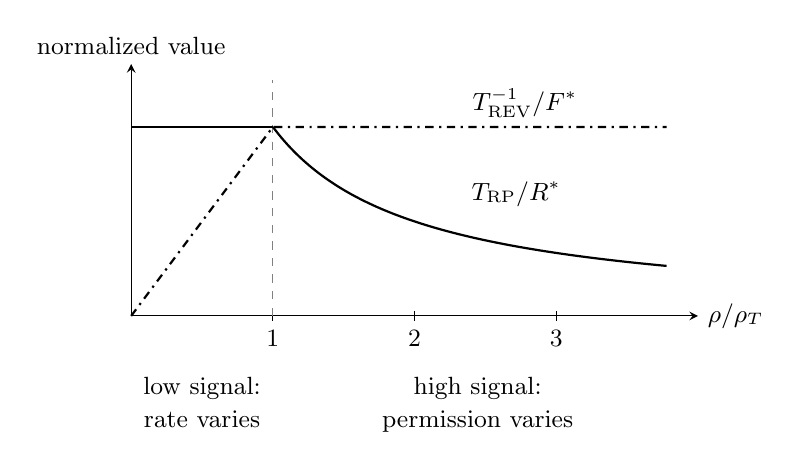
\begin{tikzpicture}[scale=1.0,>=stealth]
  \draw[->] (0,0) -- (7.2,0) node[right] {\small $\rho/\rho_T$};
  \draw[->] (0,0) -- (0,3.2) node[above] {\small normalized value};
  \foreach \x/\l in {1.8/1,3.6/2,5.4/3} {\draw (\x,0.06) -- (\x,-0.06) node[below] {\small \l};}
  \draw[dashed,gray] (1.8,0) -- (1.8,3.0);
  % T_RP / R*: flat at 1 (y=2.4) for rho<1, then 1/rho
  \draw[thick] (0,2.4) -- (1.8,2.4);
  \draw[thick,domain=1.8:6.8,samples=50,smooth] plot (\x,{2.4*1.8/\x});
  \node[right] at (4.2,1.55) {\small $\Trp/R^{*}$};
  % rate / F*: linear up to 1 then flat
  \draw[thick,dash dot] (0,0) -- (1.8,2.4) -- (6.8,2.4);
  \node[above] at (5.0,2.4) {\small $\Trev^{-1}/F^{*}$};
  \node[below,align=center] at (0.9,-0.65) {\small low signal:\\\small rate varies};
  \node[below,align=center] at (4.4,-0.65) {\small high signal:\\\small permission varies};
\end{tikzpicture}
\caption{The two signalling regimes of the one-dimensional model, normalized. Below the threshold $\rho_T$ the signal modulates the post-refractory reversal rate (dash--dotted) and the refractory period stays at $R^{*}$ (solid). Above it the rate saturates and the refractory period shortens as $1/\rho$.}
\label{fig:regimes}
\end{figure}

The distinction can be put in one sentence. In the low regime the signal changes how likely a permitted action is. In the high regime the signal changes when the action becomes permitted. Only the second is a change in the set of available actions.

\begin{definition}[Gated action set]
Let a cell have state $s=(x,\theta,r)$, with position $x$, heading $\theta$, and age $r$, and let $\sigma$ denote the signal it currently integrates. The set of actions available to it is
\[
  \A(s,\sigma) \;=\; \{\mathrm{Continue}\}\;\cup\;\{\mathrm{Reverse}\;:\; r\ge \Trp(\sigma)\},
\]
and Reverse, when in $\A$, occurs at rate $\Trev^{-1}(\sigma)$.
\end{definition}

Immediately after a reversal $r=0$ and $\mathrm{Reverse}\notin\A$. Later, $\mathrm{Reverse}\in\A$. In the high-signalling regime the boundary $\Trp(\sigma)$ moves with $\sigma$, so a strong enough signal can bring the moment of admissibility forward. The response to the signal is therefore not a map $\sigma\mapsto a$ from signal to action. It is a map from history and signal to a set of permitted actions, followed by a rate within that set. The word ``admissible'' is used here as a name for this structure. The paper itself speaks only of a refractory period and a reversal rate.

The decomposition can be written as a single hazard. For the reversal action,
\begin{equation}
  \lambda_R(t) \;=\; \mathbf{1}_{\{r(t)\ge \Trp(\sigma)\}}\;\Trev^{-1}(\sigma).
  \label{eq:hazard}
\end{equation}
Two kinds of control on an action follow. \emph{Rate control} changes the factor $\Trev^{-1}(\sigma)$ while the domain of the indicator stays fixed. \emph{Domain control} changes the threshold $\Trp(\sigma)$, and so changes the set of times at which the hazard is nonzero. The low-signalling regime is pure rate control, the high-signalling regime is domain control with the rate saturated, and the distinction is not specific to bacteria: any action with a hazard and a lockout admits the same two interventions.

\subsection{Why the boundary matters for pattern}

The paper's linear stability analysis makes the difference between the two regimes quantitative. Fluctuations are introduced around the homogeneous steady state and expanded in Fourier modes in $x$. The dominant eigenvalue $\Lambda$ depends on two dimensionless numbers: the ratio $S=\Trp/\Trev$, and a coupling $C=-\partial\log(\Trev+\Trp)/\partial\log\rho$ measuring the logarithmic sensitivity to the signal.

The result is asymmetric. In the low-signalling regime, where only the rate is modulated, $\Lambda$ stays within numerical error of zero: patterns are absent for a local-density signal and grow only very slowly for a directional-density signal. In the high-signalling regime, where the refractory period is modulated, $\Lambda$ becomes positive once $S$ is large enough, and counterpropagating waves emerge. The choice between local and directional density changes the speed of onset and the width of the parameter range, but not the qualitative picture: directional density gives a wider range of $S$ and faster emergence. The same conclusion holds in a phase-structured variant of the model, and a sufficiently nonlinear signal response can produce patterns in the low regime as well, though over a narrower range of signal levels. The paper's summary is that modulating the RP relieves the stringency on nonlinear feedback and lets patterns arise over a much broader range of signal strengths.

The mechanism they identify is synchronization. Shortening the RP at a collision allows several reversals in rapid succession, which reproduces the short-interval mode of the TBR distribution, and it aligns the reversal times of neighboring cells to the collision event. Collective structure arises from regulating when reversal becomes admissible. The paper draws an analogy to the way inhibition after firing, in networks of excitatory neurons, favors synchronization.

\section{One law, two geometries}

The one-dimensional model uses density signals, because it predates the frustration analysis and because it is tractable. The frustration hypothesis is tested in a two-dimensional agent model. Each cell is a chain of ten spheres joined by springs, driven by traction at the leading pole, with an explicit reversal of polarity. Three hypotheses are built in: (H1) reversal is triggered by frustration; (H2) both the RP and the post-refractory rate are modulated by frustration, with higher frustration giving a shorter RP and a higher rate; (H3) cells align to the ECM.

The alignment rule is where the two regimes are made different, and it is the only place. In the rippling simulation the prey matrix is represented by forcing cells to align along a fixed axis, which reduces the geometry to a quasi-one-dimensional one in which cells stay globally aligned and counterpropagating waves collide. In the swarming simulation cells align only to trails of self-deposited EPS that other cells can detect within a field of view. All other rules and parameters are shared.

The outcomes reproduce the experimental signatures without additional fitting beyond the TBR shape. The rippling simulation produces counterpropagating waves that persist for the full 500 simulated minutes, zigzag single-cell trajectories, a bimodal TBR distribution, and the enrichment of reversals at high frustration. The swarming simulation produces a network of streams that settles into a nearly stable configuration, short-ranged nematic order, a unimodal TBR distribution, and the same enrichment. Simulated frustration profiles differ between the two fields in the same direction as the data.

\begin{table}[h]
\centering
\small
\begin{tabular}{@{}lll@{}}
\toprule
 & Rippling field & Swarming field \\
\midrule
Reversal law (H1, H2) & same & same \\
Refractory modulation & same & same \\
Alignment (H3) & global axis from prey matrix & self-deposited EPS trails \\
Nematic order & long ranged & short ranged \\
TBR distribution & bimodal & unimodal \\
Mean frustration (experiment) & 0.48, sharply peaked & 0.68, broad \\
\bottomrule
\end{tabular}
\caption{The two-dimensional model varies only the alignment rule. Every other row is an outcome or a shared rule.}
\end{table}

The pattern therefore has the following logical shape. Same agent, same response law, different geometry of admissible headings, different collective state. Nothing in the cell needs to represent which regime it is in. Rippling is the name an observer gives to what the reversal machinery does when alignment is global, and swarming is the name for what it does when alignment is trail-mediated.

\subsection{The interface and sorting}

The same rules were then run in a domain split into a rippling half and a swarming half. Two patterns form, separated by a sharp and stable boundary. Cell density in the rippling half stays higher than in the swarming half regardless of the initial ratio, even when the swarming half starts with twice as many cells. Residence times explain it: cells stay in the rippling domain for a mean of 121 min per visit against 67 min in the swarming domain, consistent with the idea that repeated wave collisions interrupt forward motion and trap cells.

The reversal-defective \emph{frzE} mutant provides the test. In simulation, a 10:1 mixture of reversing and non-reversing cells behaves as one population in the swarming half, but in the rippling half the reversers make waves while non-reversers form streams and drift out, being distributed nearly uniformly across the two domains with no trapping. Experimental mixtures of wild-type and \emph{frzE} cells show the same depletion of non-reversers from the rippling field. Reversal is thus not only a rule inside a pattern. It determines who belongs to the pattern.

\section{Correlate and driver}

A methodological result in the paper deserves separate treatment because it is a clean case of a visible correlate lying downstream of the mechanism.

In rippling fields, directional density correlates with reversal. If it were the driving signal, one would expect the same in swarming, and it is not there. The paper therefore asks whether directional density could be a by-product of frustration-driven reversal together with strong one-dimensional alignment.

Simulation answers the question in both directions. When frustration is the reversal rule, reversals correlate strongly with frustration in both regimes, and correlate with directional density in rippling only, which matches the experiment. When directional density is made the reversal rule, both directional density and frustration correlate with reversal in both regimes, which is not observed, and the unimodal TBR distribution of swarming is not reproduced. Only the frustration rule reproduces the data on all counts.

Let $E_t$ denote environmental constraint (matrix alignment), $X_t$ the configuration of the whole population (positions, headings, ages), $f_t$ frustration, $R_t$ reversal, and $D_t=D(X_t)$ directional density, which is an observable of the collective configuration. An observer with access only to $D$ and $R$ sees $D\leftrightarrow R$ in rippling and is tempted to write $D\to R$. The dynamics the paper supports are instead
\[
  (E_t,X_t)\;\to\; f_t \;\to\; R_t \;\to\; X_{t+1},
  \qquad D_t = D(X_t),
\]
with feedback through $X_{t+1}$ into $f_{t+1}$. Here $D$ is not a link in a causal chain. It is a readout of the same evolving configuration that also fixes frustration, and it can correlate with $R$ because both are embedded in that configuration. Under strong one-dimensional alignment, opposed movement is concentrated at collision sites, exactly where frustration is high, so $D$ and $R$ co-vary. In swarming, alignment is short ranged, opposed movement is not concentrated, and $D$ decouples from $R$. The correlation existed because a geometry made it exist. Where the geometry is absent the correlation disappears and the mechanism, unchanged, remains.

The general point is that a statistic that predicts reversal in one condition and fails in another has failed a test that an actual driver would pass. The value of the frustration index is precisely that it passes across conditions because it is defined at the level where the mechanism operates, the discrepancy between attempted and achieved continuation, rather than at the level where the pattern becomes visible.

\section{Constraint as information}

The two features isolated at the start can now be joined. A cell has a default continuation. The environment, including other cells, sometimes makes that continuation unavailable. The discrepancy is registered as $f$. This is information generated by a failure of continuation, not a symbol supplied from outside. The cell's response to it is then not a proportional action but a change in when one particular action, reversal, becomes permitted. Constraint enters, is converted to a residual, and is applied to the timing of a gate.

\begin{remark}[Schema]
Let $g$ be the geometry of admissible headings (alignment rule) and $\phi$ the shared response law $f\mapsto(\Trp,\Trev^{-1})$. Then the paper's two-dimensional result is that the collective class $P$ is a function $P=\Pi(g;\phi)$ with $\phi$ fixed across the two conditions, and that $\Pi$ takes at least two qualitatively different values as $g$ varies. Environmental structure is doing the selecting, and it does so through $g$ and through the frustration it generates, without any instruction addressed to the agents.
\end{remark}

This suggests a way to state what an environment can do to a collective without speaking to it. It can shape which continuations fail, and where, and how often. If agents share a rule that turns failure into a timing adjustment, the environment's structure is transcribed into the collective pattern. On this reading the prey matrix is not a signal for rippling. It is a constraint field whose geometry makes frustration peaked, synchronizing, and periodic.

The structure can be made more exact by separating the environment from the information generated against it. Let $C$ be a constraint operator: it takes an attempted motion and returns what the surroundings permit, so that $v_r = C(v_t)$, where $C$ depends on the matrix and on the current positions of neighbors. Then
\[
  f \;=\; F\big(v_t,\,C(v_t)\big),
\]
with $F$ the expression in Equation~\eqref{eq:frustration}. Composing the stages gives
\[
  E \xrightarrow{\;C\;} f \xrightarrow{\;\phi\;} \A \xrightarrow{\;\lambda\;} R \xrightarrow{\;\Pi_g\;} P,
\]
where $\lambda$ is the hazard of Equation~\eqref{eq:hazard}. The operator $C$ is not communication. It does not encode $R$ or $P$, and the environment contains no message. What exists is a relation: $f$ is neither a property of the matrix nor a property of the cell, and it appears only when one acts through the other. This is the difference between information supplied by an environment and information generated against one. (The chain is a composition of stages, not a causal graph in the strict sense, since $R$ feeds back into the configuration that determines the next frustration, as in the previous section.)

Two qualifications keep the reading honest. First, it is a reading. The paper's contribution is a mechanism and its tests, and the terms gate, admissibility, and residual are imposed here to make the structure of the mechanism visible. Second, the identification of the refractory period with permission is exact in the model equations, where reversal is multiplied by a Heaviside function of age, and looser at the molecular level, where the RP is a relaxation process of RomR and FrzZ~P and not a hard prohibition.

\section{Failure changes the future}

The title can be made literal by writing the recursion in generic terms. Let $c_t$ be the state of an agent, $c^{*}_{t+1}$ the continuation it attempts, and $c_{t+1}$ the continuation realized after interaction with the environment. Define the discrepancy
\[
  \delta_t \;=\; d\big(c^{*}_{t+1},\,c_{t+1}\big)
\]
for some distance $d$. In the bacterial case the frustration index is one experimentally measurable choice of $\delta_t$, computed from velocities. What matters is not that $\delta_t>0$. It is that sufficient or accumulated discrepancy changes the next action space:
\[
  c_t \;\to\; c^{*}_{t+1} \;\to\; \delta_t \;\to\; \A_{t+1} \;\to\; c_{t+1}.
\]
A failed continuation is then not merely a miss. It is an endogenous input to the production of the next set of possible actions. In the cell, the accumulation is real and short lived: the 2D model integrates frustration over a memory of about 20 s with a kernel that weights the recent past, and the refractory period shortens as that integrated frustration rises.

The structure appears in other frameworks, including the author's own admissibility and continuation work, where an attempted continuation that meets a distinction produces the conditions of its successor. The bacterial case is not evidence for those frameworks, and no such claim is made. Its value is different. It is a biological system with an independently derived mechanism, published by others with the tests described above, that has the same abstract form, and it supplies all four terms experimentally: attempted motion, obstruction, a measurable discrepancy, and altered reversal dynamics. The general proposition it supports is this.

\begin{quote}
\emph{A constraint becomes informative when its obstruction of the present changes the space of possible next actions.}
\end{quote}

\section{Where the evidence stops}

Several limits are stated by the paper or are visible in it, and they bound the strength of the argument above.

\begin{itemize}[leftmargin=1.6em,itemsep=2pt]
  \item \textbf{Frustration is a proxy.} The authors say a direct demonstration of mechanical triggering is difficult and rely on the index as an indirect measure. Mechanosensing through the motility motors, with adaptation via FrzCD methylation, is proposed as a hypothesis and not shown. The claim that congestion is what the Frz pathway reads is therefore a well-supported inference.
  \item \textbf{The two models do not use the same signal.} The one-dimensional stability analysis is carried out with density and directional density, and the frustration hypothesis is tested only in the two-dimensional model. The stability result for RP modulation is robust to the choice of signal, which is what lets the two parts be joined, but a stability analysis for the frustration signal itself is not given. The existence of the diamond-like periodic patterns in the one-dimensional kinetic model is called an open problem.
  \item \textbf{The rippling alignment is imposed.} The prey matrix is represented by forcing a global axis, and the mechanism by which prey-derived fragments align cells is described as unknown, with a combination of physical and biochemical effects suggested. The model shows what follows from global alignment. It does not derive it.
  \item \textbf{Fitted parameters remain.} Three parameters (the frustration threshold and the steepness of the rate and RP functions) were adjusted to reproduce the TBR shape, and several others were fixed ad hoc. The aim was to reproduce the bimodal versus unimodal signature and not the means: simulated mean TBRs are 5.02 min (rippling) and 3.27 min (swarming), against 3.21 and 3.73 in the representative experiment. The ordering of the means even reverses.
  \item \textbf{Enrichment is stronger in silico.} Simulated reversals concentrate more strongly in the top frustration quartile than experimental ones. The authors show that adding noise at levels matching the tracking pipeline brings the correlations into agreement, which supports the reading of the data but also shows that the measured 50.5\,\% and 43.6\,\% are attenuated by measurement.
  \item \textbf{No claim about gene regulation is demonstrated.} That the transition needs no change in genetic regulation is a statement about sufficiency in the model, supported by the observation that cells integrate into ripples within minutes, too fast for de novo synthesis of candidate determinants. Distinct expression programs are expected to follow.
  \item \textbf{The C-signal is not excluded.} The paper argues that contact-dependent mechanical cues are more plausible than diffusible or C-signal mediation, and lists unresolved difficulties with the C-signal account, but does not formally rule out chemotaxis or other signals.
\end{itemize}

\section{Conclusion}

The central result of the paper can be stated without reference to bacteria. An agent that turns the discrepancy between attempted and achieved continuation into a time-varying permission to change direction will, under a geometry that aligns its neighbors globally, form colliding waves, and under a geometry that aligns them along their own trails, form persistent streams. The transition between the two needs only a change in the geometry, and the interface between them is stable because the same rule that generates each pattern also decides which cells remain in it.

Two easily blurred distinctions do the work. One is between a signal that is emitted and a signal that is a residual of blocked motion. The other is between a response that scales an action and a response that moves the boundary of when the action is available. Modulating the hazard inside a fixed window barely produces pattern in the paper's stability analysis, and modulating the window is what produces synchronization. The environment, meanwhile, never instructs anything. It arranges where continuation fails, and the collective learns from those failures when to turn.

\begin{thebibliography}{9}
\bibitem{saulnier2026} J.-B.~Saulnier, M.~Romanos, J.~Schrohe, C.~Cuzin, V.~Calvez and T.~Mignot, Mechanisms of spatial pattern transition in motile bacterial collectives, \emph{Nature Physics} (2026), \url{https://doi.org/10.1038/s41567-026-03416-y}.
\bibitem{guzzo2018} M.~Guzzo \emph{et al.}, A gated relaxation oscillator mediated by FrzX controls morphogenetic movements in \emph{Myxococcus xanthus}, \emph{Nat.\ Microbiol.}\ \textbf{3}, 948--959 (2018).
\bibitem{degond2018} P.~Degond, A.~Manhart and H.~Yu, An age-structured continuum model for myxobacteria, \emph{Math.\ Models Methods Appl.\ Sci.}\ \textbf{28}, 1737--1770 (2018).
\bibitem{manhart2019} A.~Manhart, Counter-propagating wave patterns in a swarm model with memory, \emph{J.\ Math.\ Biol.}\ \textbf{78}, 655--682 (2019).
\bibitem{balagam2015} R.~Balagam and O.~A.~Igoshin, Mechanism for collective cell alignment in \emph{Myxococcus xanthus} bacteria, \emph{PLoS Comput.\ Biol.}\ \textbf{11}, e1004474 (2015).
\end{thebibliography}

\end{document}
